\chapter{Architecture of Active Balancing Wireless Communication BMS}\label{ch:Architecture_Active_Balancing_BMS}
\section{Introduction}
There are plenty of topologies dedicated to the BMS active balancing, for instance, cell-to-cell charge balancing, cell-to-stack or stack-to-cell charge sharing, and stack charge sharing. Among such wide techniques cell to stack and stack-cell, charge-sharing techniques gain the upper hand because of their robustness and safety measures against the battery.
\section{Description of the Proposed Active Balancing Topologies}
\section{Active Balancing Methods}
\section{Overview of Active balancing BMS Architecture}
\section{Retrospect of BMS Hardware}
\subsubsection{Multiphase Bidirectional DC/DC Current Controller LM5170-Q1}
\indent The LM5170-q1 controller is a high precision dual channel bidirectional converter applicated in automotive 48 Volts and 12Volts dual battery systems. Depending on the Direction Signal DC/DC converter regulates the average current. The Regulated current through the DC/DC converter can be programmed by analog or Digital PWM inputs.

The LM5170-q1 has a dedicated dual channel differential current sense amplifier to monitor the current flowing through the Dc/Dc converter, which can achieve $1\%$ current sense accuracy. It has a Robust Gate driver to drive half the bridge. The Internal gate driver of the LM5170 has the capability of driving parallel MOSFET switches with a capacity of 500Watts. The synchronous diode emulation mode prevents the dc to dc converter from the negative currents and also enables the discontinuous mode of operation. This property enhances the DC/DC converter efficiency tremendously. The Controller can offer benefits of cycle-by-cycle current limitation, overVoltage protection at both low side and high side ports, Temperature protection and Mosfet failure so on...
x
\subsubsection{Matrix Switch Gate Driver :}
Modern BMS application is suffocated by the hot swapping of the Batteries for balancing. When the battery node is switched in the battery pack to balance the battery node matrix(switching circuit) the MMU will see an immense current that is flowing from the battery \cite{LTC4231_User_Datasheet}. when the switch matrix is switched to a particular node of the battery pack. The battery Node will be directly connected to the output node of the DC/DC converter (The low side of the DC/DC Converter refers to the circuit \ref{fig:Typical Bidirectional circuit of the LM5170} @low side), which will be having reservoir capacitor that will sink an immense amount of the current from the battery in very short time this will cause switching FET to burn, so it essential to switch FET very carefully. such technique is called "Hot Swap". "Hot Swap" is FET switching technique Figure\ref{fig:Mosfet_Switch_Matrix}, more often used in live power switch applications. The technique allows the gate driver circuit to monitor the current flowing through the switch circuit by the input sense resistance. By any chance Hot swap circuit doesn't allow the rapid surge of the load current in the switch circuit \cite{LTC4231_User_Datasheet}.
\paragraph{LTC4231 :}
LTC4231 is an Analog Device Inc Micro power hot-swap controller that is employed to face circuit board insertion and abrupt live power supply. An internal high-side switch driver controls the gate of an external N-channel MOSFET. Back-to-back MOSFETs can be used for reverse supply protection down to –40V \cite{LTC4231_User_Datasheet}.

The LTC4231 provides a debounce delay and allows the GATE to be ramped up at an adjustable rate. After startup, the LTC4231's quiescent current drops to 4µA during normal operation with output active. UVL, UVH, OV, and GNDSW monitor overvoltage and Undervoltage periodically, keeping total quiescent current low. Pulling SHDN low shuts down the LTC4231 and the quiescent current drops to 0.3µA.

During an overcurrent fault, the LTC4231 actively limits current while running an adjustable timer \cite{LTC4231_User_Datasheet}. The LTC4231-1 remains off after a current fault while the LTC4231-2 automatically reapplies power after a cool-down period\cite{LTC4231_User_Datasheet}.

A typical circuit diagram and the operational waveforms of the LTC4231 are described in the Figure\ref{fig: LTC4231 Application circuit and the Operational waveform}. 
For more technical details refer to the ADI LTC4231 datasheet\cite{LTC4231_User_Datasheet}.

\paragraph{Inrush Control by LTC4231 :}
In most, automotive applications keeping the inrush current low and in control is essential to avoid catastrophic damage to the switching circuits. LTC4231 takes a golden hand in controlling the inrush current by startup method (Timer Delay varying). The equations \ref{eq:LTC4321_Inrush_current} implicate the Inrush current controlled by the LTC, the Inrush current highly depends on the gate capacitance of the switch, and the output capacitance of the DC/DC capacitance (load Capacitance $C_L$). A capacitor $C_G$ of the Gate to the GND can be used to control the gate voltage slew rate for the Inrush current in the Switch.
\begin{equation}\label{eq:LTC4321_Inrush_current}
    I_{InRsush} = \frac{C_{L}}{C_{G}} \times 10\mu A
\end{equation}
\begin{figure}[h]
	\centering
	\makebox[\textwidth]{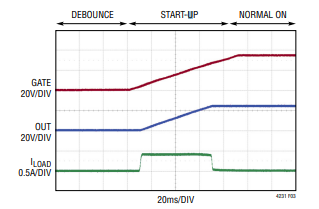
\includegraphics[width=0.9\paperwidth]{Chap04/Figures/Inrsuh_current_of_LTC4321.PNG}}
    \caption{Inrush Control by Limiting $V_{GATE}$ Slew}
    \label{fig: LTC4231 Inrush Control by Limiting VGATE Slew }
\end{figure}
The $V_{GATE}$ of the switch raise with the slope of $10\mu A/C_G$ Figure\ref{fig: LTC4231 Inrush Control by Limiting VGATE Slew}.
Once $V_{GATE}$ crosses the Vth, status goes high impedance. see the figure\cite{fig: LTC4231 Inrush Control by Limiting VGATE Slew} which explains the Inrush current protection when the $\Delta V_{Th(GATE)}$ crosses the gate voltage threshold.

The Design Example in the Chapter\ref{chap:miselleneous} explains, how to pick the design parameters to design the inrush current limit and gate driver, please follow. LTC4231 holds a wide range of advantages compared to the gate driver that is available in the market such Wide Operating Voltage Range: 2.7V to 36V, Reverse Supply Protection to –40V n Adjustable Analog Current Limit with Circuit Breaker n Automatic Retry or Latchoff on Current Fault n Overvoltage and Undervoltage Monitoring n Controls Single or Back-to-Back N-Channel MOSFETs \cite{LTC4231_User_Datasheet}. By considering all the facts we have picked the LTC4321 as the gate driver for the switch matrix.
\subsection{Current Sense :}

As elaborated in the BMS architecture High precision current sensors are used to monitor the BMS Currents. The currents are mainly monitored by the sensor charging current that is entering through the Battery pack Top and balancing current that is entering or leaving from the DC to Dc convert to the Balancing node from Battery pack TOP.

For Inventvm active balancing BMS application, The team has selected INA238 Current sensor from Texas instruments. The chapter(Current and Voltage Synchronization for BMS application) gives an extensive explanation for choosing the INA238\cite{INA238_User_Datasheet} and the application.
\subsection{Wireless Communication Hardware :}
The Bed Rock Idea behind the Inventvm active balancing BMS is to make the BMS architecture in the Wireless Communication Environment. The wireless communication architecture will reduce the immense pain of hard wires for communication in modern smart EVs. The Wireless Communication picked for the project is the Bluetooth stack, Chapter \ref{chap:BLE} takes the privilege to explain the Bluetooth Hardware choosing criteria, and design the proprietary Bluetooth solution for the projects. The BLUeNRG-355MC\cite{BLNRG355_STEVAL_GUIDE} and the Nordic\cite{NORDIC_nrf52840_USERGUIDE} are the Bluetooth solutions employed in the project.